%%%%%%%%%%%%%%%%%%%%%%%%%%%%%%%%%%%%%%%%%
% a0poster Landscape Poster
% LaTeX Template
% Version 1.0 (22/06/13)
%
% The a0poster class was created by:
% Gerlinde Kettl and Matthias Weiser (tex@kettl.de)
% 
% This template has been downloaded from:
% http://www.LaTeXTemplates.com
%
% License:
% CC BY-NC-SA 3.0 (http://creativecommons.org/licenses/by-nc-sa/3.0/)
%
%%%%%%%%%%%%%%%%%%%%%%%%%%%%%%%%%%%%%%%%%

%----------------------------------------------------------------------------------------
%	PACKAGES AND OTHER DOCUMENT CONFIGURATIONS
%----------------------------------------------------------------------------------------

\documentclass{article}[11pt]

\usepackage[svgnames]{xcolor} % Specify colors by their 'svgnames', for a full list of all colors available see here: http://www.latextemplates.com/svgnames-colors

\usepackage{graphicx} % Required for including images
\usepackage{booktabs} % Top and bottom rules for table
\usepackage[font=small,labelfont=bf]{caption} % Required for specifying captions to tables and figures
\usepackage{amsfonts, amsmath, amsthm, amssymb,subfig,cite} % For math fonts, symbols and environments
\usepackage{titlesec} % Spacing around sections

\newenvironment{myalign}{\par\nobreak\large\noindent\align}{\endalign}
\newcommand{\norm}[1]{\left\lVert#1\right\rVert}
\newcommand{\abs}[1]{\left\lvert#1\right\rvert}
\newcommand{\R}[0]{\mathbb{R}}
\newcommand{\pd}[0]{\partial}
\newcommand{\ep}[0]{\epsilon}

\titlespacing*{\section}
{0pt}{2.0ex plus 0.5ex minus .2ex}{1.0ex plus .2ex}
\titlespacing*{\subsection}
{0pt}{0.8ex plus 0.5ex minus .2ex}{0.8ex plus .2ex}
\titlespacing*{\subsubsection}
{0pt}{0.8ex plus 0.5ex minus .2ex}{0.8ex plus .2ex}
\setlength{\abovedisplayskip}{9pt}
\setlength{\belowdisplayskip}{9pt}
\setlength{\abovedisplayshortskip}{9pt}
\setlength{\belowdisplayshortskip}{9pt}

\begin{document}

%----------------------------------------------------------------------------------------
%	POSTER HEADER 
%----------------------------------------------------------------------------------------

% % The header is divided into three boxes:
% % The first is 55% wide and houses the title, subtitle, names and university/organization
% % The second is 25% wide and houses contact information
% % The third is 19% wide and houses a logo for your university/organization or a photo of you
% % The widths of these boxes can be easily edited to accommodate your content as you see fit

% \begin{minipage}[b]{0.75\linewidth}
% \veryHuge \color{NavyBlue} \textbf{A GRAPH-BASED APPROACH FOR FEATURE EXTRACTION\\ AND SEGMENTATION OF MULTIMODAL IMAGES} \color{Black}\\ % Title
% \huge \textbf{Geoffrey Iyer$^{1,2}$, Jocelyn Chanussot$^{1,2}$, and Andrea Bertozzi$^1$}\\ % Author(s)
% \huge 1. University of California, Los Angeles \\2. Univ. Grenoble Alpes, GIPSA-lab
% \end{minipage}
% %
% \begin{minipage}[b]{0.20\linewidth}
% \color{DarkSlateGray}\Large \textbf{Contact Information:}\\
% Geoffrey Iyer\\
% UCLA Mathematics Department\\ % Address
% Box 951555\\
% Los Angeles, CA 90095\\
% Email: \texttt{gsiyer@math.ucla.edu}\\ % Email address
% \end{minipage}
% %

% \vspace{1cm} % A bit of extra whitespace between the header and poster content

% %----------------------------------------------------------------------------------------


%   % ----------------------------------------------------------------------------------------
%   % ABSTRACT
%   % ----------------------------------------------------------------------------------------

%   % \color{Navy} % Navy color for the abstract

%   % \begin{abstract}
%   %   In the past few years, graph-based methods have proven to be a useful tool
%   %   in a wide variety of energy minimization problems.  In this paper, we
%   %   propose a graph-based algorithm for feature extraction and segmentation of
%   %   multimodal images. By defining a notion of similarity that integrates
%   %   information from each modality, we merge the different sources at the data
%   %   level. The graph Laplacian then allows us to perform feature extraction
%   %   and segmentation on the fused dataset. We apply this method in a practical
%   %   example, namely the segmentation of optical and lidar images. The results
%   %   obtained confirm the potential of the proposed method.
%   % \end{abstract}
%   % ----------------------------------------------------------------------------------------
%   % INTRODUCTION
%   % ----------------------------------------------------------------------------------------
%   \color{SaddleBrown} % SaddleBrown color for the introduction
%   \section*{Introduction}
%   With the increasing availability of data we often come upon problems that
%   collect data from more than once source, or \emph{modality}. To properly
%   handle these problems, we need to compare data across the different
%   modalities. The step presents a lot of difficulty, as it requires some
%   understanding of the format of the data \cite{lahat:hal-01062366}. Our goal is
%   to create a general algorithm for processing multiple modalities
%   simultaneously.

%   In this paper, we assume our datasets are co-registered (each modality
%   contains the same number of points, and they share a common indexing), as is
%   often the case in image processing problems. Our method compares graph
%   representations of each modality, extracts features in the form of
%   eigenvectors of the graph Laplacian, then applies standard data-segmentation
%   algorithms on these features to obtain a final classification.
%   % ----------------------------------------------------------------------------------------
%   % Method
%   % ----------------------------------------------------------------------------------------
%   \color{DarkSlateGray} % DarkSlateGray color for the rest of the content
%   \section{Feature Extraction}
% \label{sec:method}
% { \centering
%   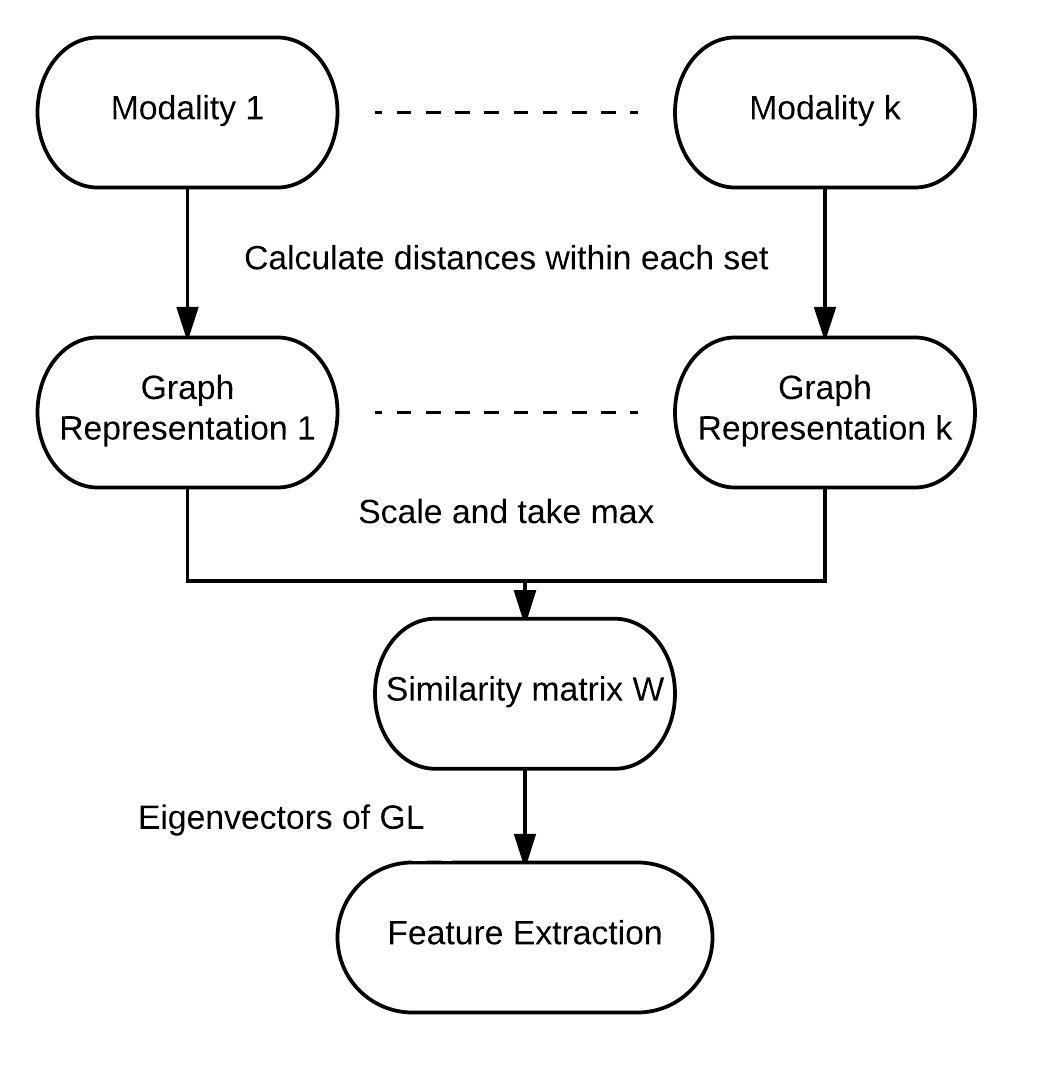
\includegraphics[width = \columnwidth]{./Images/Diagram.jpeg}
% }
% \subsection*{Graph Representation} \label{sec:GraphRep}
% \begin{itemize}\large
% \item \hspace{3mm}Datasets $X^1,X^2,\ldots,X^k$, with
%   $\abs{X^1}=\cdots=\abs{X^k}=m$.
% \item \hspace{3mm}$E^\ell = $ \emph{distance matrix}.
%   $e^\ell_{ij} = \norm{x^\ell_i - x^\ell_j}$.
% \item \hspace{3mm}$\lambda_\ell = \text{stdev}\left(E^\ell\right)$, scaling
%   factor.
% \item
%   \hspace{3mm}$X = (X^1,X^2,\ldots,X^k)\subseteq \R^{n\times
%     (dim_1+\cdots+dim_k)}$\\ the concatenated dataset.
% \item \hspace{3mm}$W = $ \emph{similarity matrix}.
%   $w_{ij} = \text{similarity between } x_i \text{ and } x_j$.
%   \begin{myalign}\label{eqn:maxNorm}
%     w_{ij} := \text{exp}\left( - \max\left(e^\ell_{ij}/\lambda_\ell\;\vert\; 1\leq\ell\leq
%         k\right)\right).
%   \end{myalign}
% \end{itemize}
% With the $\max$ norm, two nodes are considered similar only if they are similar
% in every individual modality. Heuristically, this emphasizes the unique
% information that each dataset brings.

% \subsection*{The Graph Laplacian (GL) and Eigendecomposition}\label{sec:GraphLaplacian}
% Once we have created the weights, we define the \emph{normalized graph
%   Laplacian} (GL) \cite{Mohar91}.
% \begin{myalign}\label{eqn:graphLaplacian}
%   L_{sym} = I - D^{-1/2}WD^{-1/2},
% \end{myalign}
% Where $D$ is the diagonal matrix consisting of degrees of nodes. We use the
% graph Laplacian in our energy minimizations below.

% We use the GL to solve the \emph{graph N-cut} problem. Given a partition of our
% into subsets $A_1,A_2,\ldots,A_m$, we define
% \begin{myalign}\label{eqn:NCut}\large
%   \text{NCut}(A_1,\ldots,A_m) &= \frac{1}{2}\sum_{i=1}^m
%   \frac{W(A_i,A_i^c)}{vol(A_i)}.
%   % \\ \nonumber W(A,B) &= \sum_{i\in A, j\in B} w_{ij}.  \\ \nonumber vol(A) &=
%   % \sum_{i\in A} w_{ii}.
% \end{myalign}
% Minimizing the NCut separates dissimilar nodes (the $W(A_i,A_i^c)$ term) and
% groups similar nodes (the $vol(A_i)$ term). Solving the graph min-cut problem is
% equivalent to finding an $n \times m$ indicator matrix $u$, where $u_{ij} = 1$
% if $x_i \in A_j$, and $u_{ij} = 0$ otherwise. Note that
% \begin{myalign}\large
%   \text{NCut}(A_1,\ldots,A_m) = \text{Tr}\left(u^T L_{sym} u\right).
% \end{myalign}
% Minimizing this energy is computationally infeasible \cite{Goldschmidt94}. We
% relax the problem, allowing $u$ to be an orthogonal matrix. We find
% \begin{myalign}\label{eqn:relaxedNCut}
%   \text{argmin}_{u\in \R^{n\times m}} \text{Tr}\left(u^T L_{sym}
%     u\right)\;\text{ where }u^Tu=I.
% \end{myalign}
% This problem is solved by choosing the columns of $u$ to be the $m$ eigenvectors
% of $L_{sym}$ corresponding to the $m$ smallest eigenvalues.  These eigenvectors
% are features extracted from the original dataset $X$.
% \subsection*{Example: Data Fusion Contest 2015 \cite{7536139}}
% { \centering
%   \begin{minipage}{0.45\columnwidth}
%     \centering
%     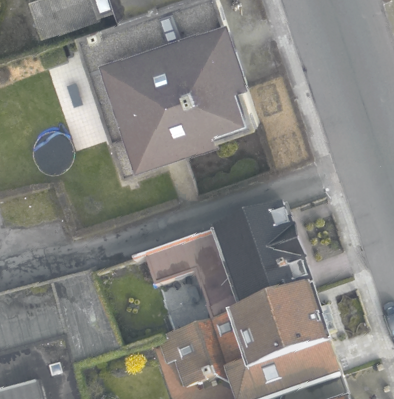
\includegraphics[width=\textwidth]{./Images/DFC2015/optical.png}%
%     \captionof{figure}{RGB Data}
%   \end{minipage}\hfill %
%   \begin{minipage}{0.45\columnwidth}
%     \centering
%     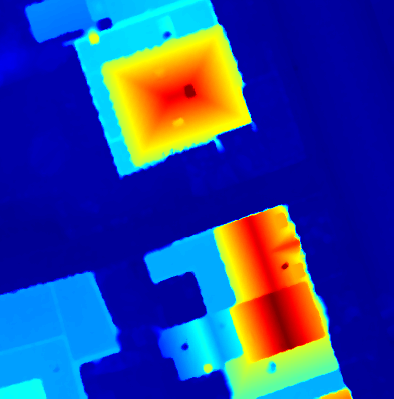
\includegraphics[width=\textwidth]{./Images/DFC2015/lidarColor.png}
%     \captionof{figure}{Lidar Data}
%   \end{minipage}
%   \label{fig:DFCfig1}
% }

% { \centering
%   \begin{minipage}{0.45\columnwidth}
%     \centering
%     
\includegraphics[width=\textwidth]{./Images/DFC2015/evec01.png}%
%     \captionof{figure}{Eigenvector 1}
%   \end{minipage}\hfill %
%   \begin{minipage}{0.45\columnwidth}
%     \centering
%     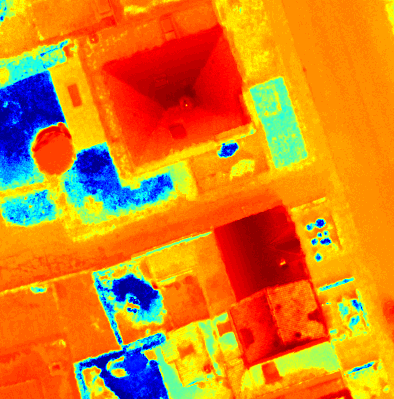
\includegraphics[width=\textwidth]{./Images/DFC2015/evec02.png}
%     \captionof{figure}{Eigenvector 2}
%   \end{minipage}
%   \label{fig:DFCfig2}
% }

% \section*{Segmentation}
% We apply two different segmentation algorithms to these features. The first is
% \emph{Spectral Clustering}, in which we directly apply $k$-means to the feature
% vectors. The second is \emph{Graph MBO}, explained below.

% \subsection*{Graph MBO}
% Here we minimize a Ginzburg-Landau energy with a semisupervised term
% \cite{Garcia2014,Merkurjev13,MERKURJEV201429}. Have $u$ an $n \times m$
% assignment matrix with
% \begin{align}
%   u_{ij} \geq 0 \; \forall i,j,\;\; \sum_{j=1}^m u_{ij} = 1.
% \end{align}
% The final output of the algorithm will be a matrix $u$ where each value is
% either $0$ or $1$. The energy we minimize is
% \begin{myalign}\label{eqn:GinzburgLandauEnergy}
%   E(u) &= \epsilon \cdot \text{Tr}\left(u^TL_{sym} u\right) +
%   \frac{1}{\epsilon}\sum_i W(u_i) \nonumber \\ &+ \sum_i
%   \frac{\mu}{2}\lambda(x_i)\norm{u_i - \hat{u}_i}^2_{L_2}.
% \end{myalign}
% The first term is the graph cut energy, similar to (\ref{eqn:NCut}). The second
% term is the multiwell potential $ W(u_i) = \prod_{k=1}^{m}\frac{1}{4}\norm{u_i - e_k}_{L_1}^2$ where $e_k$ is the $k$-th standard basis vector.  The last term includes the
% fidelity, where $\hat{u}$ represents the semisupervised input,
% \begin{align}
%   \lambda(x_i) = \begin{cases} 1 \quad \text{if $x_i$ is part of fidelity input}\\
%     0 \quad \text{else}
%   \end{cases},
% \end{align}

% We minimize this via iteritive diffusion and thresholding. If $u^{n}$ represents
% the $n$-th iterate, then to calculate $u^{n+1}$ we first diffuse
% \begin{myalign}\label{eqn:diffusion}
%   \frac{u^{n+\frac{1}{2}}-u^n}{dt} = -L_{sym} u^n - \mu \lambda(x) (u^n -
%   \hat{u}).
% \end{myalign}
% Then threshold each row
% \begin{myalign}\label{eqn:threshold}
%   u_i^{n+1} = e_r \quad \text{where }r = \text{argmax}_ju_{ij}^{n+\frac{1}{2}}.
% \end{myalign}
% The diffusion calculation can be done very efficiently by using the
% eigendecomposition of $L_{sym}$ (the feature vectors described in
% (\ref{eqn:relaxedNCut})). If we write change coordinates to the eigenbasis, then
% the diffusion step reduces to solving for coefficients
% \begin{myalign}
%   a_k^{n+1} = (1 - dt \cdot \lambda_k)\cdot a_k^n - dt\cdot d_k^n.
% \end{myalign}
% where $\lambda_k$ is the $k$-th eigenvalue of $L_{sym}$, in ascending order.

% % \subsection*{Nystr\"{o}m Extension}\label{sec:Nystrom}
% % To improve computation speed, we use Nystr\"{o}m's extension to approximate the
% % eigendecompositon of $L_{sym}$ without fully calculating the matrix
% % \cite{Fowlkes04, Merkurjev13, Woodworth13}.

% % Choose a subset $A\subset X$ of ``landmark nodes'', and have $B$ its
% % complement. Up to a permutation of nodes, we can write the weight matrix as
% % \begin{myalign}
% %   W = \begin{pmatrix} W_{AA} & W_{AB} \\ W_{BA} & W_{BB}
% %   \end{pmatrix},
% % \end{myalign}
% % % where the matrix $W_{AB} = W_{BA}^T$ consists of weights between nodes in $A$
% % % and nodes in $B$, $W_{AA}$ consists of weights between pairs of nodes in $A$,
% % % and $W_{BB}$ consists of weights between pairs of nodes in $B$.
% % Nystr\"{o}m's extension approximates $W$ as
% % \begin{myalign}
% %   W \approx \begin{pmatrix} W_{AA} \\ W_{BA} \end{pmatrix}
% %   W_{AA}^{-1} \begin{pmatrix} W_{AA} & W_{AB}\end{pmatrix}.
% % \end{myalign}
% % It is possible to find $\abs{A}$ approximate eigenvectors of $W$ using only the
% % matrices $W_{AA},W_{AB}$, so our matrices are of size at most
% % $\abs{A}\times\abs{X}$, rather than $\abs{X}\times\abs{X}$.
% % ----------------------------------------------------------------------------------------
% % Results
% % ----------------------------------------------------------------------------------------
% \subsection*{Results: Data Fusion Contest 2015 \cite{7536139}}
% \label{sec:DFCexperiment}

% % { \centering
% %   \begin{minipage}{0.45\columnwidth}
% %     \centering
% %     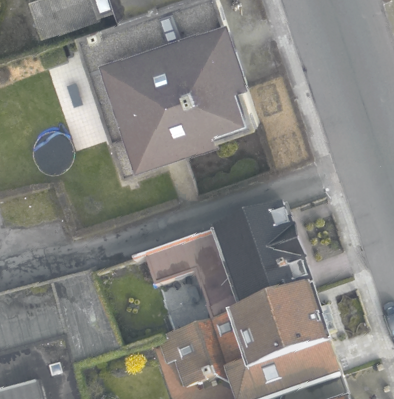
\includegraphics[width=\textwidth]{./Images/DFC2015/optical.png}%
% %     \captionof{figure}{RGB Data}
% %   \end{minipage}\hfill %
% %   \begin{minipage}{0.45\columnwidth}
% %     \centering
% %     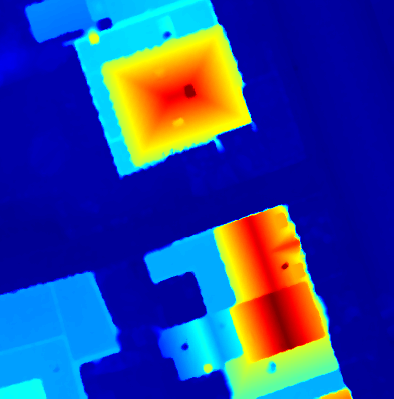
\includegraphics[width=\textwidth]{./Images/DFC2015/lidarColor.png}
% %     \captionof{figure}{Lidar Data}
% %   \end{minipage}
% %   \label{fig:DFCfig1}
% % }

% { \centering
%   \begin{minipage}{0.45\columnwidth}
%     \centering
%     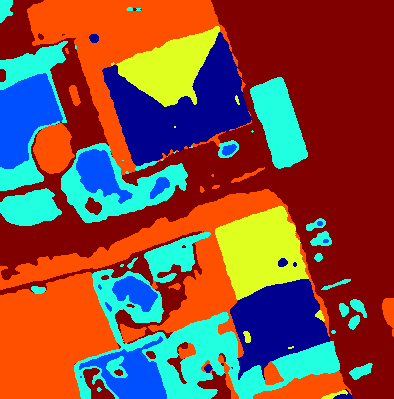
\includegraphics[width=\textwidth]{./Images/DFC2015/specClust.png}%
%     \captionof{figure}{Spectral Clustering}
%   \end{minipage}\hfill %
%   \begin{minipage}{0.45\columnwidth}
%     \centering
%     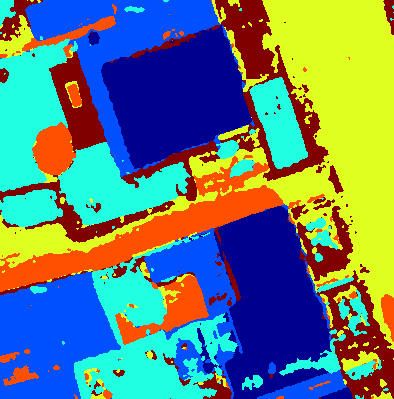
\includegraphics[width=\textwidth]{./Images/DFC2015/MBO.png}
%     \captionof{figure}{Graph MBO}
%   \end{minipage}
%   \label{fig:DFCfig2}
% }

% % In figure \ref{fig:DFCevec1}, \ref{fig:DFCevec2} we show two example
% % eigenvectors of the graph Laplacian. As explained in \ref{sec:SpecClust},
% % these vector can be thought of as feature of our dataset, and looking at them
% % will give us a rough idea of the final segmentation. Notice how in
% % \ref{fig:DFCevec1} the dark-grey asphalt is distinct from both the nearby
% % grass (which is at the same elevation), and the roofs of the buildings (which
% % are a similar color). This shows at the feature level that our algorithm is
% % successfully using both the optical and the lidar data when determining what
% % pixels can be considered similar. The difference shown in this example vector
% % then causes the classification algorithm to separate those regions in the
% % final results \ref{fig:DFCspecClust}, \ref{fig:DFCMBO}.

% \subsection*{Results: Umbrella Data \cite{Scharstein14}}
% \label{sec:UmbrellaExperiment}

% { \centering
%   \begin{minipage}{0.45\columnwidth}
%     \centering
%     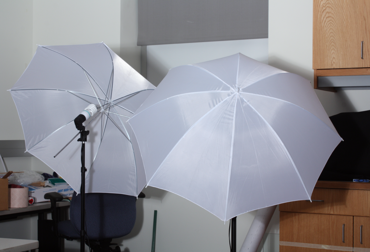
\includegraphics[width=\textwidth]{./Images/Umbrella/optical.png}%
%     \captionof{figure}{RGB Data}
%   \end{minipage}\hfill %
%   \begin{minipage}{0.45\columnwidth}
%     \centering
%     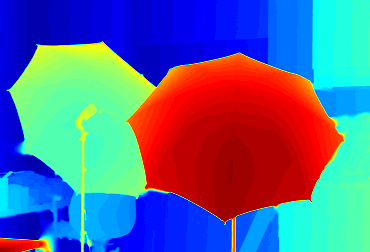
\includegraphics[width=\textwidth]{./Images/Umbrella/lidarColor.png}
%     \captionof{figure}{Lidar Data}
%   \end{minipage}
%   \label{fig:Umbrellafig1}
% }

% { \centering
%   \begin{minipage}{0.45\columnwidth}
%     \centering
%     
\includegraphics[width=\textwidth]{./Images/Umbrella/evec01.png}%
%     \captionof{figure}{Eigenvector 1}
%   \end{minipage}\hfill %
%   \begin{minipage}{0.45\columnwidth}
%     \centering
%     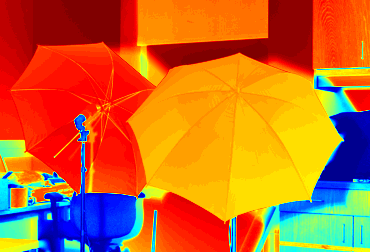
\includegraphics[width=\textwidth]{./Images/Umbrella/evec02.png}
%     \captionof{figure}{Eigenvector 2}
%   \end{minipage}
%   \label{fig:Umbrellafig1}
% }

% { \centering
%   \begin{minipage}{0.45\columnwidth}
%     \centering
%     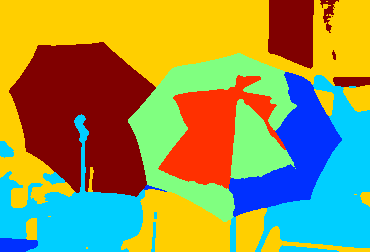
\includegraphics[width=\textwidth]{./Images/Umbrella/specClust.png}%
%     \captionof{figure}{Spectral Clustering}
%   \end{minipage}\hfill %
%   \begin{minipage}{0.45\columnwidth}
%     \centering
%     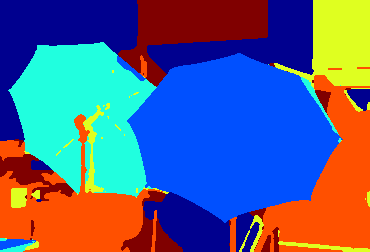
\includegraphics[width=\textwidth]{./Images/Umbrella/MBO.png}
%     \captionof{figure}{Graph MBO}
%   \end{minipage}
%   \label{fig:DFCfig2}
% }

% % In fig \ref{fig:Umbrella} we show the results of our method applied to another
% % optical/lidar set (found in \cite{Scharstein14}), which we will refer to as
% % the umbrella data. Similar to the DFC set, the umbrella data serves as a good
% % example because it cannot be easily analyzed using one modality alone. The
% % umbrellas and the background walls are nearly the same shade of white, and can
% % only be distinguished in the lidar data. Meanwhile, the different pieces of
% % the background all lie at nearly the same depth, and can only be separated by
% % color. As was the case with the DFC data, the final classifications
% % \ref{fig:UmbrellaSpecClust}, \ref{fig:UmbrellaMBO} can be understood by
% % looking at the individual feature vectors. The first example eigenvector
% % \ref{fig:UmbrellaEvec1} mimics the lidar data, but with addition detail drawn
% % from the optical image. For example, this eigenvector differentiates the black
% % umbrella stand from the actual umbrella, even though both objects are at the
% % same depth. The second example eigenvector \ref{fig:UmbrellaEvec2} groups
% % together all the background objects with a darker hue.

% \subsection*{Results: Jade Plant Data \cite{Scharstein14}}

% { \centering
%   \begin{minipage}{0.45\columnwidth}
%     \centering
%     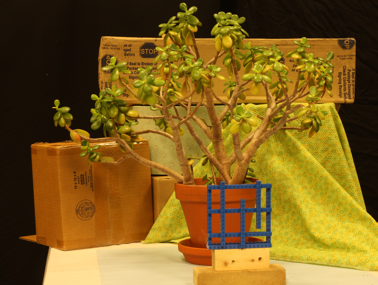
\includegraphics[width=\textwidth]{./Images/Jadeplant/optical.png}%
%     \captionof{figure}{RGB Data}
%   \end{minipage}\hfill %
%   \begin{minipage}{0.45\columnwidth}
%     \centering
%     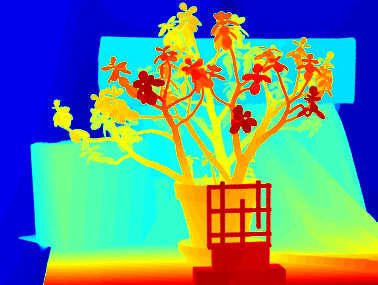
\includegraphics[width=\textwidth]{./Images/Jadeplant/lidar.png}
%     \captionof{figure}{Lidar Data}
%   \end{minipage}
%   \label{fig:Jadeplantfig1}
% }

% { \centering
%   \begin{minipage}{0.45\columnwidth}
%     \centering
%     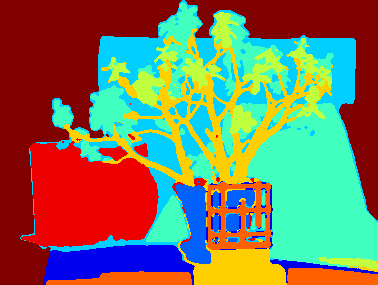
\includegraphics[width=\textwidth]{./Images/Jadeplant/specClust.png}%
%     \captionof{figure}{Spectral Clustering}
%   \end{minipage}\hfill %
%   \begin{minipage}{0.45\columnwidth}
%     \centering
%     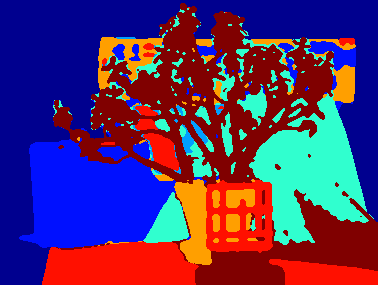
\includegraphics[width=\textwidth]{./Images/Jadeplant/MBO.png}
%     \captionof{figure}{Graph MBO}
%   \end{minipage}
%   \label{fig:DFCfig2}
% }

% % Found in the same paper as the umbrella data \cite{Scharstein14}, we test our
% % method against another optical/lidar scene of a jade plant. In figure
% % \ref{fig:Jadeplant} we once again display our classification result along with
% % several example eigenvectors. As before, we can see in each eigenvector some
% % pieces of the final classification.

% % \section*{Conclusions}
% % \label{sec:conclusions}
% % Graph-based methods provide a straightforward and flexible method of combining
% % information from multiple datasets. By considering the similarity between points
% % in each individual dataset, we are able to directly compare the different
% % modalities.

% % Our next area of interest is to generalize the method by removing or weakening
% % the co-registration assumption. In our experiment we only consider cases where
% % pixels correspond exactly between images. We could not, for example, process two
% % images taken from different angles. If we remove this assumption the algorithm
% % could be applied to data fusion problems across a much larger number of fields.

% \section*{Acknowledgments}\label{sec:Acknowledgements}

% This work was supported by NSF grant DMS-1118971, ONR grant N00014-16-1-2119,
% NSF grant DMS-1417674, European Research Council (Grant no. 320684 - CHESS
% project), and CNRS (Grant no. PICS-USA 263484)

% ----------------------------------------------------------------------------------------
%\newpage
%
%\nocite{*} % Print all references regardless of whether they were cited in the poster or not
\bibliographystyle{acm} % Plain referencing style
\bibliography{../../BibTex/research} % Use the example bibliography file sample.bib

\end{document}